%!TEX root = ../../thesis.tex
\chapter{Mark and Sweep}
\label{cha:mark-sweep}
Wir beginnen mit einer Vorstellung des ersten Garbage-Collection-Algorithmus, der auf John \textsc{McCarthy} zurückgeht \cite[191--193]{mccarthy1960}.
Im Rahmen eines im Jahr 1960 veröffentlichten Artikels über die Berechnung rekursiver Funktionen auf dem \textit{IBM 704} mithilfe des \textit{LISP Programming Systems} erläutert McCarthy die Speicherung von Daten in einer Listenstruktur.
Diese besteht aus Paaren, deren erster Eintrag \texttt{car} die zu speichernde Information enthält, während im zweiten Eintrag \texttt{cdr} die Registeradresse des nachfolgenden Paares zu finden ist.
Register, die aktuell nicht zur Speicherung von Daten genutzt werden, befinden sich in einer \textit{free storage list}.
Bei der Anforderung von Speicher für ein zu speicherndes Datum werden Register aus dieser Liste entfernt.
Durch die Manipulation der Registeradressen können Paare verwaisen, was zu Speicherlecks führt.
Zur Auflösung dieser Problematik bietet LISP als erste Programmiersprache ihrer Zeit eine automatische Speicherverwaltung, die von McCarthy wie folgt grob umschrieben wird:
Im Falle von Speicherknappheit wird -- ausgehend von einer Menge von Basisregistern -- ermittelt, welche Register über eine Folge von \texttt{cdr}-Einträgen erreichbar sind.
Nicht erreichbare Register enthalten überschreibbare Inhalte, sodass diese zurück in die \textit{free storage list} eingefügt werden können und wieder als freie Speicherplätze zu Verfügung stehen.
Diese zweischrittige Vorgehensweise -- das Erkennen nicht mehr benötigter Speicherbereiche und die anschließende Freigabe eben jener -- bildet die Grundlage des \textit{Mark-and-Sweep}-Algorithmus.

\section{Naives Mark and Sweep}
\label{sec:naive-mark-sweep}
Der naive Mark-and-Sweep-Algorithmus arbeitet in zwei Schritten:
Zunächst wird bestimmt, welche Objekte im Speicher unerreichbar sind, weil sie von keinem anderen erreichbaren Objekt referenziert werden.
Diese Objekte können gefahrlos freigegeben werden, da auf ihre Informationen nicht mehr zugegriffen werden kann.
Der zweite Schritt besteht aus einer Traversierung des gesamten Heaps.
Dabei werden alle existierenden Objekte besucht und diejenigen freigegeben, die im ersten Schritt als unerreichbar identifiziert werden konnten.
Die entsprechenden Speicherbereiche stehen anschließend wieder für neue Objekte zu Verfügung.

\begin{algorithm}
\begin{algorithmic}[1]
	\State \MethodHead{collectGarbage}():
	\State \quad \Method{markStart}()
	\State \quad \Method{sweepHeap}()
	\State
	\State \MethodHead{markStart}():
	\State \quad \Var{toDo} $\gets$ $\emptyset$				\Comment{Noch abzuarbeitende Objekte}
	\State \quad \FOREACH \Var{obj} $\in \Roots$		\Comment{Beginne mit Basisobjekten}
	\State \quad \quad \IF \Method{isNotMarked}(\Var{obj})
	\State \quad \quad \quad \Method{setMarked}(\Var{obj})	\Comment{Objekt als erreichbar markieren}
	\State \quad \quad \quad \Method{add}(\Var{toDo}, \Var{obj})	
	\State \quad \quad \quad \Method{mark}()			\Comment{Abarbeitung starten}
	\State
	\State \MethodHead{mark}():
	\State \quad \WHILE \Var{toDo} $\neq \emptyset$
	\State \quad \quad \Var{obj} $\gets$ \Method{remove}(\Var{toDo})			\Comment{Hole nächstes Objekt}
	\State \quad \quad \FOREACH \Var{adr} $\in \Pointers(\Var{obj})$	\Comment{Hole nächste Referenz auf Objekt}
	\State \quad \quad \quad \IF (\Var{adr} $\neq$ \Null $\wedge$ \Method{isNotMarked}(\Var{*adr}))	
	\State \quad \quad \quad \quad \Method{setMarked}(\Var{*adr})	
	\State \quad \quad \quad \quad \Method{add}(\Var{toDo}, \Var{*adr})
\end{algorithmic}
\caption[Naives Mark and Sweep -- Markierung]{Naives Mark and Sweep -- Markierung (vgl. \cite[Kap. 2.2]{jones-lins})}
\label{algo:naive-mark}
\end{algorithm}

Die Markierungsphase (engl. \textit{mark}) funktioniert wie folgt:
Zunächst wird mittels der Methode \Method{markStart} eine Menge \Var{toDo} erzeugt, die diejenigen Objekte enthält, die bereits als erreichbar erkannt wurden, aber selbst noch nicht verarbeitet wurden (Zeile 6 in Algorithmus~\ref{algo:naive-mark}).
In diese werden alle bislang unmarkierten Basisobjekte der Menge \Roots eingefügt und markiert, da sie in jedem Fall erreichbar sind (Zeile 7 bis 10).
Ist ein Basisobjekt bereits markiert worden, so wurde es schon entdeckt -- etwa, weil es durch ein zuvor abgearbeitetes Objekt referenziert wird.
Daraus folgt, dass es ebenfalls bereits abgearbeitet wurde oder sich noch in der Menge \Var{toDo} befindet.
In beiden Fällen muss es folglich nicht erneut zu \Var{toDo} hinzugefügt werden.

Bereits nach dem Hinzufügen des ersten Basisobjekts wird die Methode \Method{mark} aufgerufen, welche die \Var{toDo}-Menge abarbeitet.
Für jedes Objekt in \Var{toDo} werden diejenigen Felder betrachtet, die eine Referenz auf ein Objekt enthalten (Zeile 15 und 16).
Wenn dieses Objekt noch nicht markiert wurde, wird es in diesem Augenblick zum ersten Mal entdeckt.
Da es somit erreichbar ist, kann es markiert und zu \Var{toDo} hinzugefügt werden, um zu einem späteren Zeitpunkt abgearbeitet zu werden (Zeile 17 und 18).
Verweist die Referenz hingegen auf ein Objekt, das bereits markiert wurde, wurde dieses schon zuvor entdeckt.
Auch hier ist ein erneutes Hinzufügen zu \Var{toDo} überflüssig.
Sobald \Var{toDo} leer ist, erfolgt die Rückkehr zur Methode \Method{markStart}, sodass ggfs. das nächste Basisobjekt abgearbeitet wird.

\todo[inline]{Kleines Beispiel hier, großes in den Anhang?}

Es ist wesentlich, dass Objekte bereits markiert werden, wenn sie der Menge \Var{toDo} hinzugefügt werden, und nicht etwa, nachdem sie abgearbeitet wurden (Zeile 9 und 10 bzw. 18 und 19).
Andernfalls besteht bei zyklischen Referenzen die Gefahr einer Endlosschleife, da unmarkierte Objekte mehrfach hinzugefügt würden.
Präziser können wir festhalten, dass \Var{toDo} zu jedem Zeitpunkt ausschließlich bereits markierte Objekte enthält.
Da keine Objekte hinzugefügt werden, die bereits markiert wurden (Zeile 8 und 16), wird kein Objekt doppelt verarbeitet.
Da zudem mit jeder Iteration der \WHILE-Schleife mindestens ein Objekt aus \Var{toDo} entfernt wird (Zeile 15), die Anzahl aller Objekte endlich ist und wir voraussetzen, dass während der Ausführung des Garbage Collectors keine neuen Objekte entstehen, wird sowohl die \WHILE-Schleife, als auch die \FOREACH-Schleife nach endlich vielen Schritten terminieren.

Anstatt die Abarbeitung der \Var{toDo}-Menge zu beginnen, sobald das erste Basisobjekt erfasst wurde, können statt dessen auch zunächst alle Basisobjekte zu \Var{toDo} hinzugefügt und die Methode \Method{mark} im Anschluss aufgerufen werden.
Je nachdem, wie \Var{toDo} in der Praxis realisiert wird -- zum Beispiel in Form eines Stacks -- kann damit die Traversierung der Objekte beeinflusst werden.
Dies kann einen erheblichen Einfluss auf die Performanz der Markierungsphase haben, wenn Caching-Effekte eine Rolle spielen. \todo{evtl. später genauer drauf eingehen}

\begin{algorithm}
\begin{algorithmic}[1]
	\State \MethodHead{sweep}():
	\State \quad \Var{pos} $\gets$ \Method{nextObject}(\Var{HEAP\_START})
	\State \quad \WHILE \Var{pos} $\neq$ \Null
	\State \quad \quad \IF \Method{isMarked}(\Var{*pos})
	\State \quad \quad \quad \Method{unsetMarked}(\Var{*pos})
	\State \quad \quad \ELSE \Method{free}(\Var{pos})
	\State \quad \quad \Var{pos} $\gets$ \Method{nextObject}(\Var{pos})
\end{algorithmic}
\caption[Naives Mark and Sweep -- Bereinigung]{Naives Mark and Sweep -- Bereinigung (vgl. \cite[Kap. 2.2]{jones-lins})}
\label{algo:naive-sweep}
\end{algorithm}

Die Bereinigungsphase (engl. \textit{sweep}) beginnt unmittelbar nach der Markierungsphase durch Aufruf der Methode \Method{sweep}.
Die Variable \Var{pos} wird mit der Speicheradresse initialisiert, an der sich das erste Objekt im Heap befindet.
Wir gehen davon aus, dass eine Methode \Method{nextObject} zu Verfügung steht, die anhand einer übergebenen Speicheradresse die Adresse des nachfolgenden Objektes oder \Null zurückgibt, wenn dieses nicht existiert.
Dadurch wird der Heap linear traversiert; nicht markierte Objekte werden freigegeben, während die Markierung erreichbarer Objekte zurückgesetzt wird.

Wir halten zunächst fest, dass der Mark-and-Sweep-Algorithmus in seiner Gänze terminiert und korrekt ist, sofern während der Garbage Collection das laufende Programm angehalten wird:

\begin{mybox}
\begin{satz}
	\label{satz:mark-sweep-correctness}
	Der Mark-and-Sweep-Algorithmus terminiert und ist korrekt, wenn der Mutator während der Arbeit des Kollektors angehalten wird.
\end{satz}
\end{mybox}

\begin{proof}
	Wie oben erläutert, terminiert die Markierungsphase in jedem Fall, da bei angehaltenem Mutator keine neuen Objekte erstellt werden.
	Gleiches gilt für die Bereinigungsphase, in der alle Objekte des Heaps in endlicher Zeit besucht werden.
	Somit terminiert der gesamte Algorithmus.
	
	Weiter werden lediglich nicht markierte Objekte freigegeben (Zeile 4--6 in Algorithmus~\ref{algo:naive-sweep}).
	Bleibt ein Objekt \code{obj} unmarkiert, so ist \code{obj} kein Basisobjekt, da \Method{markStart} alle Basisobjekte markiert.
	Somit wird kein Basisobjekt freigegeben.
	Wir zeigen, dass es nach der Markierungsphase zudem keine zwei Objekte $\Var{a}$, $\Var{b}$ mit $\Var{a} \rightarrow \Var{b}$ gibt, sodass $\Var{a}$ markiert und $\Var{b}$ unmarkiert ist:
	Da $\Var{a}$ markiert ist, wurde $\Var{a}$ auch der Menge $\Var{toDo}$ hinzugefügt (Zeile 9f bzw. 18f in Algorithmus~\ref{algo:naive-mark}).
	Entsprechend gab es eine Iteration der \WHILE-Schleife mit $\Var{obj} = \Var{a}$.
	Gilt nun \Var{a} $\rightarrow$ \Var{b}, so ist $\Var{\&b} \in \Pointers(\Var{a})$.
	Folglich wird in einer Iteration der \FOREACH-Schleife mit \Var{adr} $=$ \Var{\&b} auch \Var{*(\&b)} $=$ \Var{b} markiert, falls \Var{b} nicht schon zuvor markiert wurde.
	Es existiert somit keine Referenz von einem erreichbaren auf ein unmarkiertes Objekt, weswegen keine erreichbaren Objekte freigegeben werden.
\end{proof}

Die Bedingung, dass der Mutator während des Markierens pausiert wird, ist tatsächlich notwendig, um zu vermeiden, dass fälschlicherweise keine erreichbaren Objekte entfernt werden, wie folgendes Beispiel zeigt (vgl. \cite[969]{dijkstra1978}):
Betrachten wir etwa die Situation, dass zwei Basisobjekte $\Var{A}$ und $\Var{B}$ alternierend auf ein Objekt $\Var{C}$ verweisen, das ausschließlich über $\Var{A}$ oder $\Var{B}$ erreichbar ist.
Während der Kollektor aktiv ist, führe der Mutator folgenden Code aus:

\begin{center}
\begin{minipage}{0.3\textwidth}
	\centering
	\begin{algorithmic}[1]
		\State \Var{B.ref} $\gets$ \Var{\&C}
		\State \Var{A.ref} $\gets$ \Null
		\State \Var{A.ref} $\gets$ \Var{\&C}
		\State \Var{B.ref} $\gets$ \Null
	\end{algorithmic}
\end{minipage}~
\begin{minipage}{0.3\textwidth}
	\centering
	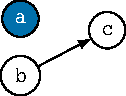
\includegraphics[keepaspectratio]{img/tikz/ch2-concurrent1.pdf}
\end{minipage}~
\begin{minipage}{0.3\textwidth}
	\centering
	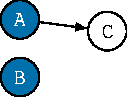
\includegraphics[keepaspectratio]{img/tikz/ch2-concurrent2.pdf}
\end{minipage}
\end{center}

Es könnte passieren, dass der Kollektor gerade Objekt $\Var{A}$ abarbeitet, unmittelbar nachdem Zeile~2 ausgeführt wurde.
Es wird dann keine Referenz auf Objekt $\Var{C}$ vorgefunden.
Wenn der Kollektor nun Objekt $\Var{B}$ betrachtet, nachdem bereits Zeile~4 abgearbeitet wurde, wird Objekt $\Var{C}$ weiterhin nicht entdeckt.
Insgesamt wird Objekt $\Var{C}$ somit nicht markiert, obwohl es erreichbar ist.
In der Folge würde $\Var{C}$ irrtümlich freigegeben werden, sodass im schlimmsten Fall ein hängender Zeiger entsteht oder sogar Datenverlust verursacht wird -- der Algorithmus arbeitet also nicht korrekt.

Algorithmen, die zur Vermeidung von \textit{race conditions} zwischen Kollektor und Mutator die Arbeit des letzteren unterbrechen, werden auch als \textit{Stop-the-World-Algorithmen} bezeichnet.

\section{Markierungsmöglichkeiten}
\label{sec:marking-methods}
Da das Anhalten des Mutators während eines gesamten Garbage-Collection-Zyklus zu vergleichsweise großen Verzögerungen führt, ist eine Optimierung der Markierungsphase zielführend.
Wünschenswert ist, Kollektor und Mutator möglichst häufig eine nebenläufige Ausführung zu ermöglichen, ohne dabei die Korrektheit der Garbage Collection zu gefährden.
Wir haben gesehen, dass die Manipulation von Referenzen während der Markierungsphase dazu führt, dass Verweise von markierten auf unmarkierte Objekte entstehen können, sodass erreichbare Objekte unmarkiert bleiben.
Um dies zu vermeiden, könnte man als ersten Ansatz auf die Idee kommen, beim Schreiben einer neuen Referenz in ein Feld eines Objekts das Ziel dieser Referenz sofort zu markieren.
Dies ist jedoch nur scheinbar eine Lösung:
Da das Ziel ebenfalls Referenzen auf unmarkierte Objekte bereithalten könnte, entstehen dadurch möglicherweise neue Referenzen von markierten auf unmarkierte Objekte.
Von Dijkstra et al. stammt ein Ansatz, der diese Idee aufgreift und um ein \textit{Zwischenstadium} erweitert \cite[S. 969f]{dijkstra1978}.
Diese ermöglicht es, markierte Objekte, die bereits komplett abgearbeitet wurden, von solchen zu unterscheiden, die bislang lediglich entdeckt wurden.
Dazu werden Objekte mit drei verschiedenen Farben markiert:

\begin{description}
	\item[weiß:] Das Objekt wurde bislang nicht als erreichbar identifiziert.
		Bleibt es nach Ende der Markierungsphase weiß, kann es freigegeben werden.
	\item[grau:] Das Objekt ist erreichbar, allerdings wurden die Felder des Objekts noch nicht auf Referenzen zu weiteren Objekten überprüft.
	\item[schwarz:] Das Objekt ist erreichbar und alle Felder des Objekts wurden bereits überprüft.
\end{description}

Zu Beginn des Algorithmus sind alle existierenden Objekte weiß.
Wir modifizieren den ursprünglichen Mark-and-Sweep-Algorithmus~\ref{algo:naive-mark} so, dass Objekte bei ihrer Entdeckung grau und nach Abarbeitung ihrer Felder schwarz markiert werden.
Hierfür existiert eine atomare Prozedur \Method{setColor}, die die Markierung eines Objekts auf eine bestimmte Farbe \Var{WHITE}, \Var{GRAY} oder \Var{BLACK} setzt.
Auf diese Art bleiben nicht mehr erreichbare Objekte weiß und können anschließend als löschbar identifiziert werden.
Analog wird die \Method{sweep}-Prozedur in Algorithmus~\ref{algo:naive-sweep} so abgeändert, dass Objekte gelöscht werden, wenn sie weiß markiert sind.
Andernfalls wird ihre Markierung zurück auf weiß gesetzt.

\begin{algorithm}[h]
\begin{algorithmic}[1]
	\Pre Alle Objekte sind weiß markiert.
	\State \MethodHead{markStart}():
	\State \quad \Var{graySet} $\gets$ $\emptyset$				\Comment{Grau markierte Objekte}
	\State \quad \FOREACH \Var{obj} $\in \Roots$
	\State \quad \quad \IF \Method{isWhite}(\Var{obj})
	\State \quad \quad \quad \Method{setColor}(\Var{obj}, \Var{GRAY})	
	\State \quad \quad \quad \Method{add}(\Var{graySet}, \Var{obj})	
	\State \quad \quad \quad \Method{mark}()
	\Statex
	\State \MethodHead{mark}():
	\State \quad \WHILE \Var{graySet} $\neq \emptyset$
	\State \quad \quad \Var{obj} $\gets$ \Method{remove}(\Var{graySet})
	\State \quad \quad \Method{setColor}(\Var{obj}, \Var{BLACK})		\Comment{Objekt wird nun abgearbeitet}
	\State \quad \quad \FOREACH \Var{adr} $\in \Pointers(\Var{obj})$
	\State \quad \quad \quad \IF (\Var{adr} $\neq$ \Null $\wedge$ \Method{isWhite}(\Var{*adr}))	
	\State \quad \quad \quad \quad \Method{setColor}(\Var{*adr}, \Var{GRAY})	\Comment{Referenzierte Objekte grau markieren}
	\State \quad \quad \quad \quad \Method{add}(\Var{graySet}, \Var{*adr})
	\Statex
	\State \MethodHead{sweep}():
	\State \quad \Var{pos} $\gets$ \Method{nextObject}(\Var{HEAP\_START})
	\State \quad \WHILE \Var{pos} $\neq$ \Null
	\State \quad \quad \IF \Method{isWhite}(\Var{*pos})
	\State \quad \quad \quad \Method{free}(\Var{pos})
	\State \quad \quad \ELSE \Method{setColor}(\Var{*pos}, \Var{WHITE})
	\State \quad \quad \Var{pos} $\gets$ \Method{nextObject}(\Var{pos})
\end{algorithmic}
\caption[Markierung mit Drei-Farben-Abstraktion]{Markierung mit Drei-Farben-Abstraktion (vgl. \cite[S. 970]{dijkstra1978})}
\label{algo:tricolor}
\end{algorithm}

Mithilfe dieser \textbf{Drei-Farben-Abstraktion} (engl. \textit{tri-color abstraction}) können wir nun Referenzmanipulationen zulassen, die parallel zur Markierungsphase der Garbage Collection stattfinden:
Wird in einem Objekt \Var{a} eine Referenz auf ein Objekt \Var{b} hinterlegt, so kann dies dazu führen, dass \Var{b} erreichbar wird.
Infolgedessen müssen auch alle von \Var{b} referenzierten Objekte als erreichbar identifiziert werden.
Somit ist es zielführend, \Var{b} beim Setzen der Referenz grau zu markieren und zu \Var{graySet} hinzuzufügen, sofern dies noch nicht der Fall ist oder die Felder von \Var{b} bereits verfolgt wurden.
Dies kann etwa mit einer \textit{Schreibbarriere} (engl. \textit{write barrier}) realisiert werden, die genau dann zum Einsatz kommt, wenn eine Referenz in ein Feld eines Objektes geschrieben wird (siehe Algorithmus~\ref{algo:tricolor-barrier}).
Auf diese Art kann es jedoch vorkommen, dass Objekte unerreichbar werden, nachdem sie bereits grau oder schwarz markiert wurden.
Entsprechend verbleiben sie im Speicher und werden erst im nächsten Garbage-Collection-Zyklus entfernt.

\begin{algorithm}
\begin{algorithmic}[1]
	\Input Objekt \Var{obj}, in dem Referenz gesetzt wird; Index des Feldes \Var{i}; zu setzende Referenz \Var{ref}
	\State \Atomic \MethodHead{writeRef}(\Var{obj}, \Var{i}, \Var{ref}):
	\State \quad \Var{obj[i]} $\gets$ \Var{ref}
	\State \quad \IF (\Var{ref} $\neq$ \Null $\wedge$ \Method{isWhite}(\Var{*ref}))
	\State \quad \quad \Method{setColor}(\Var{*ref}, \Var{GRAY})
	\State \quad \quad \Method{add}(\Var{grayList}, \Var{*ref})
\end{algorithmic}
\caption[Schreibbarriere zur Manipulation von Referenzen]{Schreibbarriere zur Manipulation von Referenzen in Objekten.}
\label{algo:tricolor-barrier}
\end{algorithm}

An dieser Stelle gehen wir auf die Terminierung und Korrektheit des modifizierten Mark-and-Sweep-Algorithmus ein.

\begin{mybox}
\begin{satz}
	Der Mark-and-Sweep-Algorithmus mit Drei-Farben-Abstraktion terminiert und ist korrekt, sofern während der Arbeit des Kollektors keine neuen Objekte erzeugt werden.
\end{satz}
\end{mybox}

\begin{proof}
	\textit{Zur Terminierung:} Wir halten zunächst fest, dass Objekte während der Markierungsphase ausschließlich \textit{dunkler} gefärbt werden:
	In Algorithmus~\ref{algo:tricolor} werden lediglich weiß markierte Objekte grau gefärbt (Zeile~5 und 14); eine Weißfärbung geschieht in dieser Phase grundsätzlich nicht.
	Analog zum ursprünglichen Algorithmus~\ref{algo:naive-mark} enthält \Var{graySet} nur grau markierte Objekte.
	Jedes Objekt befindet sich dadurch höchstens einmal in dieser Menge.
	Da \Var{graySet} nach jeder Iteration der \WHILE-Schleife um ein Objekt reduziert wird und keine neuen Objekte erzeugt werden, terminieren auch hier \WHILE- und \FOREACH-Schleife nach endlich vielen Schritten.
	Zuletzt terminiert auch Bereinigungsphase (siehe Satz~\ref{satz:mark-sweep-correctness}).
	
	\textit{Zur Korrektheit:} Erneut ist zu zeigen, dass keine Objekte unmarkiert bleiben, die erreichbar sind.
	Dies wäre genau dann der Fall, wenn nach der Markierungsphase ein schwarz markiertes Objekt eine Referenz auf ein weiß markiertes Objekt besitzt.
	Wir zeigen daher die Gültigkeit folgender Schleifeninvariante für die \WHILE-Schleife:
	\begin{description}
		\item[(A)] Es existieren keine zwei Objekte \Var{a} und \Var{b} mit \Var{a} $\rightarrow$ \Var{b}, sodass \Var{a} schwarz markiert und \Var{b} weiß markiert ist.
	\end{description}
	Da zu Beginn laut Vorbedingung alle Objekte weiß markiert sind und bis zum Eintritt in die \WHILE-Schleife Objekte nur grau markiert werden, gilt (A) trivialerweise, da keine schwarz markierten Objekte existieren.
	Gelte nun (A) zu Beginn einer Schleifeniteration und sei \Var{a} dasjenige Objekt, das der Menge \Var{graySet} entnommen und schwarz gefärbt wird (Zeile~10f).
	Existiert nun ein weiteres Objekt \Var{b} mit \Var{a} $\rightarrow$ \Var{b}, so ist \Var{\&b} $\in \Pointers(\Var{a})$.
	Ist \Var{b} bereits grau oder schwarz markiert, so geschieht nichts.
	Andernfalls wird \Var{*(\&b)} $=$ \Var{b} grau markiert (Zeile~14).
	In beiden Fällen ist \Var{b} am Ende der Schleife nicht weiß markiert.
	Da \Var{a} das einzige Objekt ist, das in dieser Iteration schwarz gefärbt wird, ist (A) nach der Iteration weiterhin gültig.
	Da die Schleife terminiert, die Invariante aufrecht erhalten bleibt und in der Bereinigungsphase nur weiß markierte Objekte freigegeben werden, ist der Algorithmus korrekt.
\end{proof}

\todo[inline]{Markierungsmöglichkeiten (Tricolor, Bitmapping); Lazy Sweeping}